\documentclass[12pt]{book}

\usepackage[utf8]{inputenc}
\usepackage[T1]{fontenc}
\usepackage{geometry}
\usepackage{graphicx}
\usepackage[spanish]{babel}
\usepackage{amsthm}
\usepackage{amsmath}
\usepackage{amssymb}
\usepackage{calrsfs}
\usepackage{trfsigns}

\newtheorem{thm}{Teorema}[section]
\theoremstyle{definition}
\newtheorem{dfn}{Definición}[section]
\theoremstyle{remark}
\newtheorem{note}{Nota}[section]
\theoremstyle{plain}
\newtheorem{lem}[thm]{Lema}

\geometry{letterpaper}



\title{Ejercicios de control}
\author{Dr. Casimiro Gómez González\\
	Facultad de Electrónica, UPAEP\\
               correo: casimiro.gomez@upaep.mx\\
               Tel: 222 229 9428}
\date{Primavera 2010}

\begin{document}
\frontmatter
\maketitle
\chapter{Prólogo}
Material de Ejercicios con sus respectivas soluciones, para prepararse para las evaluaciones parciales

\tableofcontents

\mainmatter

\chapter{Ejercicios para el primer Parcial}

\section{Ejercicios de Euler-Lagrange}

\subsection{Caída de dos eslabones}
\label{p4}
Dos eslabones sin masa de longitud $2r$, cada uno con una masa $m$ fija en la mitad estan unidas por sus extremidades. Una sobre la otra, como se muestra en la figura. El extremo inferior de la masa de abajo esta unida al suelo por medio de una bisagra. Los eslabones se mantienen de tal forma que el eslabón inferior se coloca verticalmente, y el eslabon superior tiene un pequeño ángulo $\varepsilon$ con respecto de la vertical. Luego los eslabones se sueltan. En ese instante, ¿cual es la aceleración angular de los dos eslabones? considera despues que $\varepsilon$ es muy pequeña.
\begin{figure}
\centering
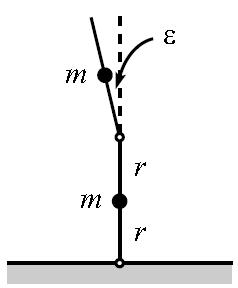
\includegraphics[width=1in]{doseslabones.jpeg}
\caption{Figura para el problema \ref{p4}}
\label{fig4}
\end{figure}

\subsubsection{Solución}

Para la solución de este problema hay que obtener las coordenadas de cada una de las masas que se encuentran en la mitad de los eslabones en un instante cualquiera despues de que se soltaron y estan cayendo

\subsection{Caída de tres eslabones}
\label{p1}
Tres eslabones sin masa, de longitud $2 r$, cada uno con una masa $m$ fija en la mitad, están unidos en sus extremos como se muestra en la figura. El extremo inferior del eslabón mas bajo esta unido al suelo a través de una bisagra. Los eslabones están sostenidos de tal forma que los dos eslabones inferiores estan verticales, y el eslabón superior tienes un pequeño ángulo $\varepsilon$ respecto de la vertical. Posteriormente los eslabones se sueltan. En este instante, ¿cual es la aceleración angular de los tres eslabones? Posteriormente considera que $\varepsilon$ es muy pequeño.

\begin{figure}
\centering
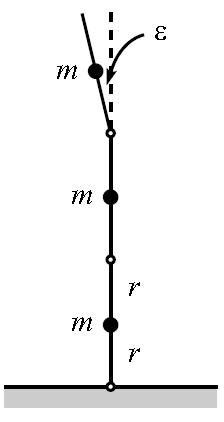
\includegraphics[width=1in]{treseslabones.jpeg}
\caption{Figura para el problema \ref{p1}}
\label{fig1}
\end{figure}



\subsection{Plano en movimiento}
\label{p2}
Un bloque de masa $m$ se mantiene sin movimiento en un plano sin fricción de masa $M$ y con un ángulo de inclinación $\theta$ (ver figura ). El plano descansa en una superficie horizontal sin fricción. Cuando el bloque se suelta ¿Cual es la aceleración horizontal del plano?
\begin{figure}
\centering
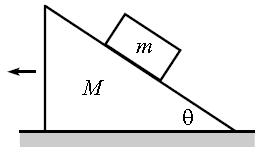
\includegraphics[width=3in]{planomoviendose.jpeg}
\caption{Figura para el problema \ref{p2}}
\label{fig2}
\end{figure}

\subsubsection{Solución}
Se proponen dos variables cada una indicando el desplazamiento del plano inclinado y del bloque.
La solución de este problema es

\begin{equation*}
\label{equ1}
\begin{aligned}
M \ddot{x_1} + m ( \ddot{x_1} + \ddot{x_2}) \tan ^2 \theta = m g \tan \theta \\
m \ddot{x_2}+m  ( \ddot{x_1} + \ddot{x_2}) \tan ^2 \theta = m g \tan \theta
\end{aligned}
\end{equation*}

\begin{figure}
\centering
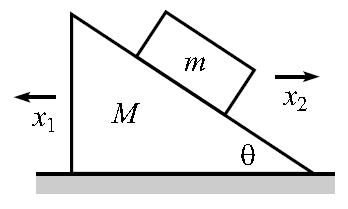
\includegraphics[width=2in]{solucionplano.jpeg}
\caption{Figura de la solución  para el problema \ref{p4}}
\label{fig6}
\end{figure}

\subsection{Dos masa unidas por un cable}
\label{p3}
Dos masa iguales, $m$ conectadas por un cable, cuelgan sobre dos poleas (de tamaño despreciable), como se muestra en la figura .  La masa de la izquierda se mueve verticalmente, pero la derecha se mueve oscilando (en el plano que forman las masas y las poleas). Encontrar la ecuación de movimiento para $r$ y $\theta$.

\begin{figure}
\centering
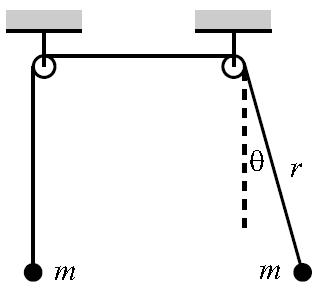
\includegraphics[width=2in]{poleas.jpeg}
\caption{Figura para el problema \ref{p3}}
\label{fig3}
\end{figure}

Supongase que la masa de la izquierda inicia en reposo, y la masa de la derecha presenta pequeñas oscilaciones con una amplitud angular $\varepsilon$ (con $\varepsilon \ll 1$). ¿Cual es la aceleración promedio inicial (promedio de pocos periodos de oscilación) de la masa izquierda? ¿En cual dirección se mueve?

\subsubsection{Solución}
\begin{equation*}
\label{equ2}
\begin{aligned}
2 \ddot{r} = r \dot{\theta}^2 -g (1- \cos \theta) \\
\frac{d}{d t}(r^2 \dot{\theta})= -g r \sen \theta
\end{aligned}
\end{equation*}
 La primera ecuación calcula las fuerzas y las aceleraciones en la dirección de la cadena. La segunda ecaución relaciona el torque debido a la gravedad con el cambio en el momento angular de la masa derecha

\subsection{Doble péndulo}
\label{p5}
Considere un doble péndulo hecho de dos masas $m_1$ y $m_2$ y dos cuerdas de longitud $l_1$ y $l_2$. Encontrar las ecuaciones de movimiento.

\begin{figure}
\centering
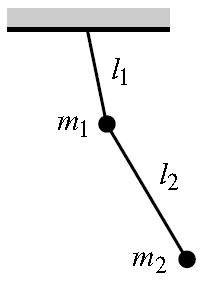
\includegraphics[width=1.2in]{doblependulo.jpeg}
\caption{Figura para el problema \ref{p5}}
\label{fig5}
\end{figure}

\subsubsection{Solución}
La solución de este problema es la siguiente
\begin{equation*}
\label{equ2}
\begin{aligned}
0 & = (m_1 + m_2) l_1 ^2 \ddot{\theta_1} + m_2 l_1 l_2 \ddot{\theta _2} \cos(\theta _1 - \theta _2) + m_2 l_1 l_2 \dot{\theta _2}^2 \sen (\theta _1 - \theta _2) + (m_1 + m_2) g l_1 \sen \theta _1\\
0 & =  m_2 l_2 ^2 \ddot{\theta_2} + m_2 l_1 l_2 \ddot{\theta _1} \cos(\theta _1 - \theta _2) - m_2 l_1 l_2 \dot{\theta _1}^2 \sen (\theta _1 - \theta _2) +  m_2 g l_2 \sen \theta _2
\end{aligned}
\end{equation*}


\backmatter
\end{document}
